% The example is similar to the one given in pgf manual at: https://ftp.cc.uoc.gr/mirrors/CTAN/graphics/pgf/contrib/pgfplots/doc/pgfplots.pdf (page 567)

\documentclass[border=2pt]{standalone}

% Drawing 
\usepackage{tikz}
\usetikzlibrary{3d, shapes.multipart}

% Styles
\tikzset{>=latex} % for LaTeX arrow head
\tikzset{axis/.style={black, thick,->}}
\tikzset{vector/.style={>=stealth,->}}
\tikzset{every text node part/.style={align=center}}

% Notation
\usepackage{amsmath} % for \text
 
\begin{document}

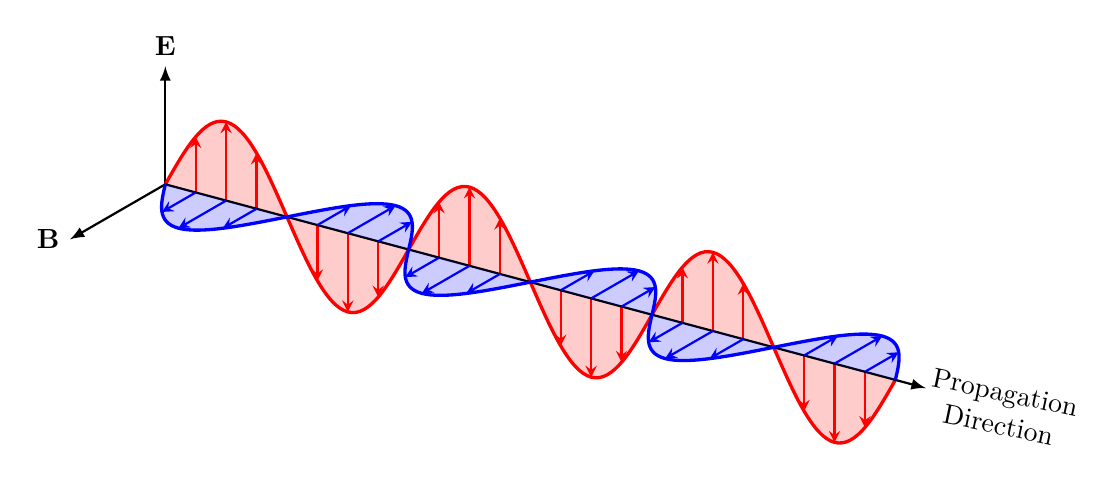
\begin{tikzpicture}[x={(-150:0.7)}, y={(90:1.0)}, z={(-15:8mm)}]

% Wave Function
\def\wave{
	\draw[fill, very thick, fill opacity=.2]
	     (0,0) sin (1,1) cos (2,0) sin (3,-1) cos (4,0)
	           sin (5,1) cos (6,0) sin (7,-1) cos (8,0)
	           sin (9,1) cos (10,0) sin (11,-1) cos (12,0);
         
	\foreach \shift in {0,4,8}
	{
		\begin{scope}[xshift=\shift cm,thin]
		        \draw[-stealth, thick] (.5,0)  -- (0.5,0 |- 45:1cm);
		        \draw[-stealth, thick] (1,0)   -- (1,1);
		        \draw[-stealth, thick] (1.5,0) -- (1.5,0 |- 45:1cm);
		        \draw[-stealth, thick] (2.5,0) -- (2.5,0 |- -45:1cm);
		        \draw[-stealth, thick] (3,0)   -- (3,-1);
		        \draw[-stealth, thick] (3.5,0) -- (3.5,0 |- -45:1cm);
		 \end{scope}
	} 
}

% Red Wave
\begin{scope}[canvas is zy plane at x=0, draw=red, fill=red] 
	\draw[-latex, thick, black] (0,0) -- (0, 1.5) node[above] {$\mathbf E$};
	\wave
\end{scope}

% Blue Wave
\begin{scope}[canvas is zx plane at y=0, draw=blue, fill=blue]
	%% Direction of Propagation
	\draw[-latex, thick, black] (0,0) -- (12.5, 0) node[rotate = -12, pos=1.1] {Propagation\\Direction};
	\draw[-latex, thick, black] (0,0) -- (0,2) node[left] {$\mathbf B$};
	\wave
\end{scope}

\end{tikzpicture}

\end{document}